\documentclass{sigchi}

\pagenumbering{arabic}% Arabic page numbers for submission. 

% Use \toappear{...} to override the default ACM copyright statement (e.g. for preprints).

% Load basic packages
\usepackage{balance}  % to better equalize the last page
\usepackage{graphics} % for EPS, load graphicx instead
 \usepackage{times}   %comment if you want LaTeX's default font
\usepackage[hyphens]{url}      % llt: nicely formatted URLs


% llt: Define a global style for URLs, rather that the default one
\makeatletter
\def\url@leostyle{%
  \@ifundefined{selectfont}{\def\UrlFont{\sf}}{\def\UrlFont{\small\bf\ttfamily}}}
\makeatother
\urlstyle{leo}


\usepackage{etoolbox}
\makeatletter
\patchcmd{\maketitle}{\@copyrightspace}{}{}{}
\makeatother


% To make various LaTeX processors do the right thing with page size.
\def\pprw{8.5in}
\def\pprh{11in}
\special{papersize=\pprw,\pprh}
\setlength{\paperwidth}{\pprw}
\setlength{\paperheight}{\pprh}
\setlength{\pdfpagewidth}{\pprw}
\setlength{\pdfpageheight}{\pprh}

% Make sure hyperref comes last of your loaded packages, 
% to give it a fighting chance of not being over-written, 
% since its job is to redefine many LaTeX commands.
\usepackage[pdftex]{hyperref}
\hypersetup{
pdftitle={Contextual privacy and security in the data life cycle for big data systems Vigneswaren, Palmer},
pdfauthor={Vigneswaren, Palmer},
pdfkeywords={big data, contextual privacy, contextual security},
bookmarksnumbered,
pdfstartview={FitH},
colorlinks,
citecolor=black,
filecolor=black,
linkcolor=black,
urlcolor=black,
breaklinks=true,
}

% create a shortcut to typeset table headings
\newcommand\tabhead[1]{\small\textbf{#1}}

% End of preamble. Here it comes the document.
\begin{document}

\title{Contextual Privacy and Security in the Data Life Cycle for Big Data Systems}

% Note that submissions are blind, so author information should be omitted
\numberofauthors{2}
\author{
  \alignauthor Kapil Haresh Vigneswaren\\
    \affaddr{David Cheriton School of Computer Science}\\
    \affaddr{University of Waterloo}\\
    \affaddr{Waterloo, ON, Canada, N2L 3G1}\\
    \email{khvignes@uwaterloo.ca}\\
  \alignauthor Andrew Palmer\\
    \affaddr{David Cheriton School of Computer Science}\\
    \affaddr{University of Waterloo}\\
    \affaddr{Waterloo, ON, Canada, N2L 3G1}\\
    \email{a9palmer@uwaterloo.ca}\\
}

% Teaser figure can go here
%\teaser{
%  \centering
%  \includegraphics{Figure1}
%  \caption{Teaser Image}
%  \label{fig:teaser}
%}

\maketitle

\begin{abstract}
Several characteristics of big datasets open up many new avenues for exploitation, and as such, new privacy and security models are required to address these emerging challenges. The magnitude of datasets generated make it near impossible for data managers to capture all the contextual semantics relevant to a unit of data, and this causes novel difficulties in privacy and security of these big data systems. At the micro-level, a datum in any software system transitions between several phases, from inception to deletion; this is known as the data life cycle, which provides a concrete guide for tracking the many states of a unit of data. The usefulness of such a model only increases with the complexity of the system that it represents, so it is useful to examine privacy and security from this perspective, as it provides a precise framework for discussion. This paper provides practical privacy and security recommendations for every step of the data life cycle, examining prominent infrastructures and their features that relate to their data management policies.
\end{abstract}

\keywords{
	big data, contextual privacy, contextual security, data life cycle}

\section{1. Introduction}

Big Data represents a paradigm shift in computing where datasets are becoming too voluminous, diverse, and unpredictable for traditional computing models to handle efficiently. As a result, new computing frameworks are rapidly being developed and adopted, with the focus shifting from a centralized platform towards a more distributed one. Big data naturally yields insights into new types of information on a level more granular and voluminous than any previous computing paradigms. Large volumes of data are great in theory, however in the context of big data, there are naturally more opportunities for exploitation, whether intentional or not. 

In a world that is increasingly reliant on data, it is the ethical duty of organizations to be proactive about privacy and security and to be informed of the potential risks they expose to their customers to. In one study, the average loss in share price over a three-day period, after news of a security breach, was nearly 5.6 percent, representing \$17-28 million for some companies \cite{garg2003quantifying}. Thus, knowledge about these risks represents a good motivator, as it is a financially sound investment for organizations.

Contextual privacy and security are essential standards to be maintained in big data systems, but can prove to be very difficult to maintain in the existing implementations. The goal of this paper is to provide an analysis of privacy and security issues at each step of the data life cycle as it relates to the contextual characteristics of the data under question.

\textbf{Contributions.} This paper makes the following contributions:
\begin{itemize}
  \item Explores the importance of contextual privacy and security in big data systems
  \item Creates a concrete guide with a set of best practices that are of practical use to developers of big data systems, which ensures that the privacy and security of users are preserved.
  \item Identifies existing big data software systems, and their potential weaknesses in relation to contextual privacy and security.
\end{itemize}

\section{2. Preliminaries}
\subsection{Big Data}

The concept of big data is quite vague and evolving very rapidly, given the vast amount of research that the area has seen in recent times. As a result, there have been several proposed definitions from the community since its coinage.

The most widely-cited definition comes from a Meta (now Gartner)  report from 2001, which introduced three prominent V's associated with big data: volume, velocity, and variety \cite{laney20013d}. These terms refer to the increasing size of datasets, the increasing rate at which data is produced, and the increased heterogeneity of data formats, respectively. This classic definition is concrete, however we feel that to a first-time reader, the essence of the idea is not sufficiently communicated. In a survey of definitions, Laney identifies and explores several interpretations of big data \cite{laney20013d}. He also recognizes the classic definition however concludes that the majority of big data definitions comprise a mixture of the following elements:

\begin{enumerate}
\item \textit{Size}, which refers to the volume of the data.
\item \textit{Complexity}, which refers to the structure, behavior and permutations of the data.
\item \textit{Technologies}, which are the tools and techniques that are used to process large and/or complex datasets.
\end{enumerate}

Laney concludes by extrapolating the aforementioned factors and postulates that big data always describes ``the storage and analysis of large and or complex datasets using a series of techniques including, but not limited to: NoSQL, MapReduce and machine learning''. We find this definition best captures the essence of big data, however for clarity, and precision, this paper will examine big data against the classic V's.

\subsection{Context}

The definition we find most intuitive, by Dey et al., describes context as ``any information that can be used to characterize the situation of an entity'', where an entity is ``a person, place, or object that is considered relevant to the interaction between a user and an application, including the user and applications themselves''\cite{abowd1999towards}.

Dey et al. suggest that simply, context is ``any information that can be used to characterize the situation''.

Furthermore, context can be divided into four categories \cite{chen2000survey}:

\begin{enumerate}
\item \textit{Computing context}, which encompasses things like network connectivity, communication cost, and communication bandwidth.

\item \textit{User context}, which captures details about the user, such as location, surroundings, and social situation.

\item \textit{Physical context}, which involves the physical surroundings, e.g. noise, temperature, traffic conditions, etc.

\item \textit{Temporal context}, which, as it suggests, deals with time, e.g. the time of day, the current month, the current season, etc.

\end{enumerate}

Nissenbaum suggests that the relevant user contexts for privacy, are things such as canonical activities, roles, relationships, power structures, norms (or rules), and internal values \cite{nissenbaum2009privacy}.

\subsection{Privacy}

One of the first discussions around consumer data privacy and data protection was by Alan Westin, in 1968 who described privacy as ``the claim of individuals, groups, or institutions to determine for themselves when, how, and to what extent information about them is communicated to others'' \cite{westin1968privacy}. Viewed in terms of the relation of the individual to social participation, privacy is the voluntary and temporary withdrawal of a person from the general society through physical or psychological means, either in a state of solitude or small group intimacy or, when among large groups, in a condition of anonymity or reserve
\cite{westin1968privacy}.

Due to a heavier reliance on computing technologies, the amount of sensitive data collected about individuals has 
reached unprecedented levels, and will only continue to grow in the future. Naturally, with larger amounts of sensitive data, comes a greater risk for exploits by third parties, which include governments, but also corporations, law enforcement agents, family and friends as well as strangers \cite{scuPrivacyDefine}.

One scenario where sensitive data can be exploited is in the case of an online banking system where users are assigned unique client card numbers that they may use for online payments. Given enough data, third parties could perform sufficient analysis to reverse-engineer personally-identifying details about users, including their purchasing preferences, spending habits, medical history and even family history. 

Another worrying aspect is that privacy can still be violated regardless of whether or not a person directly uses an electronic or internet-connected device; this is the case of many seemingly harmless face-to-face transactions. For example, a person physically performs a transaction at a bank, or collects their medication from a pharmacy, in both of these cases it is likely that their photo ID is required prior to the transactions. The issue with these scenarios is that both the bank and the pharmacy may rely on electronic management systems and central data stores. Although the central data stores of a bank may not be connected to the pharmacy's, assuming that one is able to gain access to the data in transit or once it is stored in the data store of both companies, given sufficient time, one could still analyze the datasets and identify if the same user who had the mortgage also goes to collect prescription medication - which in turn, once the frequency of the person going to collect the medication is identified, could allow a third party to make conclusions that this particular person has a chronic disease that could lead to them not being able to pay off that mortgage. 

\subsection{Security} Security, on the other hand, is quite different from privacy. Security is defined as the prevention or protection against access to information by unauthorized recipients, or unauthorized (but intentional) destruction or alteration of that information itself \cite{schell2006webster}. Another concept of security is that it is the ability of a system to protect information and system resources to ensure the preservation of three factors: confidentiality, integrity and availability \cite{2_ross_2000}. These are known as the three pillars of security is defined as follows:
\begin{itemize}
\item \textbf{Confidentiality} - Unauthorized access of information is prevented
\item \textbf{Integrity} - Information isn't modified in any way by unauthorized users in any way, such that an authorized user will not be able to detect this modification
\item \textbf{Availability} - Ensuring the availability of a system, should this be violated, it would be said that there's a "denial of service" attack taking place.
\end{itemize}
In some cases, it is argued that authentication, instead of availability is the third pillar of security, however this is argued to be incorrect in many cases as Authentication is technically part of the Confidentiality pillar. It is possible to have a system that is not able to guarantee one's privacy despite being mathematically/theoretically ``secure'', however this is not very common, in many cases a violation of security will violate one's privacy as well as potentially sensitive data is now accessible to someone who isn't supposed to be able to access it.
\pagebreak
\subsection{Issues with Big Data}
In the context of big data systems, security is something that is pretty tough to ensure. To understand the difficulty of this, we take a look at the 3 V's of big data systems: volume, velocity and variety \cite{gewirtz_2016} \cite{haughngibilisco_2014}.
\begin{itemize}

\item \textbf{Volume:} In a traditional data system, a handful of machines may be sufficient to process the volume of data. However, big data systems require much larger clusters of computational resources with potentially hundreds of thousands of machines networked across the globe and datasets on the scale of petabytes. For some context, in 2014, Amazon Web Services, one of the premier cloud systems in the world was estimated to have 1.5 to 2 million servers \cite{clark_2016}; no doubt, this number is probably much larger now. Figures on this scale were unprecedented in the context of traditional data systems.

\item \textbf{Velocity:} Because of the increased number of sources of data, there are significantly larger amounts of new data processed every second, day in, day out. Furthermore, the rate at which data is collected is accelerating and has a multiplicative effect on the total volume of data.

For example, consider that in 2014, Amazon AWS data centers were allocated up to 102 Tb/sec of incoming bandwidth (this data was back in 2014 and it would be fair to say that this has likely increased) and within the data center itself, there is a significantly higher bandwidth. Cumulatively, this velocity of data represents a magnitude of volume at unprecedented levels (even assuming that only 50\% of the bandwidth being used) \cite{morgan_2014}. Ensuring the preservation of security while maintaining this velocity of data transfer in and out is one of the toughest challenges.

\item \textbf{Variety:} The other thing that should be considered is the variety of the data in big data systems. Unlike traditional data systems, which are generally designed for specific kinds of data, big data systems have data incoming in a variety of formats, from various sources \cite{haughngibilisco_2014}. As a result, security solutions for such heterogeneous datasets need to take into account the variability of the data that the systems handle.
\end{itemize}

When large scale privacy and security violations occur, the after effects are somewhat similar to what happens in small scale systems, however, the effects are magnified. While in small scale systems, only a small fraction of the population of users may be affected, in big data systems, the number of users  affected can run into the millions, or billions \cite{yahooHack}. Securus Technologies is a good example in this case, as they were the leading provider for phone services for many of the prisons and jails in the United States \cite{smithlee_2015}. In 2015, there was a massive security breach that violated the privacy of inmates, as over 70 million records of phone calls, complete with links to the recordings of the phone calls itself, spanning a period of slightly over 2 years. While it did have some benefit, as the breach revealed that some conversations between the inmates and attorneys were recorded (which is illegal), it did violate the privacy of many inmates who had been serving their time. The hack is an indication of how much information that is often stored on big data systems, and the worst part is that it not only affects those who are in prison, but the countless people who are connected to them. The irony was that Securus Technologies markets itself as a company that is able to provide a superior phone system (the Secure Call Platform), that is able to allow for call monitoring and secure storage of the recordings of the calls itself. The fact that the breach could even take place is a clear indication that the system which stored such large amounts of data was more vulnerable than what it claimed to be. The scale of a  single hack can affect a large number of people and is one of the main issues with security and privacy in the context of big data system.

\section{3. Contextual Privacy and Security}

Contextual security, or context-aware security, is the idea where the context of the data is used to make security decisions \cite{8_rouse_2013} \cite{10_peterson_2015}. It allows for better, more tailored security decisions to be made. In our context, this allows us to tailor the security measures to be put into place as data moves along the life cycle. Big data systems will require different security protocols given that data will go through many transformations and be distributed between traditional security domains.

Contextual privacy to some extent has a similar definition to contextual security; the extent of which is that information under one context should not be shared in the same way as information under a different one. For example, one may approve their data to be used for a particular purpose at a specific time, but doesn't allow the storage system to use the data for a different purpose, or at a different time \cite{9_wangtan_2013}. Considering the amount of analysis possible with big data systems, it is possible for such violations to take place. Contextual privacy is an issue because it encapsulates sensitive information that may not be immediately obvious since the dangers may not be immediately apparent from the data itself. As such, it should be handled as mandated by the necessary legal regulations and organizational policies. The key concern for contextual privacy is data misappropriation, which is a type of misconduct that is the result of acts that modify the context of data to an inappropriate one \cite{sayaf2015contextual}.

Unfortunately, since context is an abstract construct, existing frameworks often do not take into account the extra information required to identify data misappropriation. Countering cases of misappropriation is difficult in current implementations, since they are limited only to prohibiting or allowing certain actions. These approaches are unable to take into account the appropriateness of the state of data after undergoing a particular action.

Some researchers suggest that big data systems should include the enforcement of a data policy in order for them to be processed on trusted systems, while complying with other external requirements, i.e., context \cite{demchenkobig}. Such a requirement also needs to support all stages of the life cycle, and a solution may including a mechanism for policy attachment to data that ensures persistence of the policies that require enforcement, especially with continuous online and offline processing.

\section{4. Data Life Cycle}
\begin{figure}[ht]
    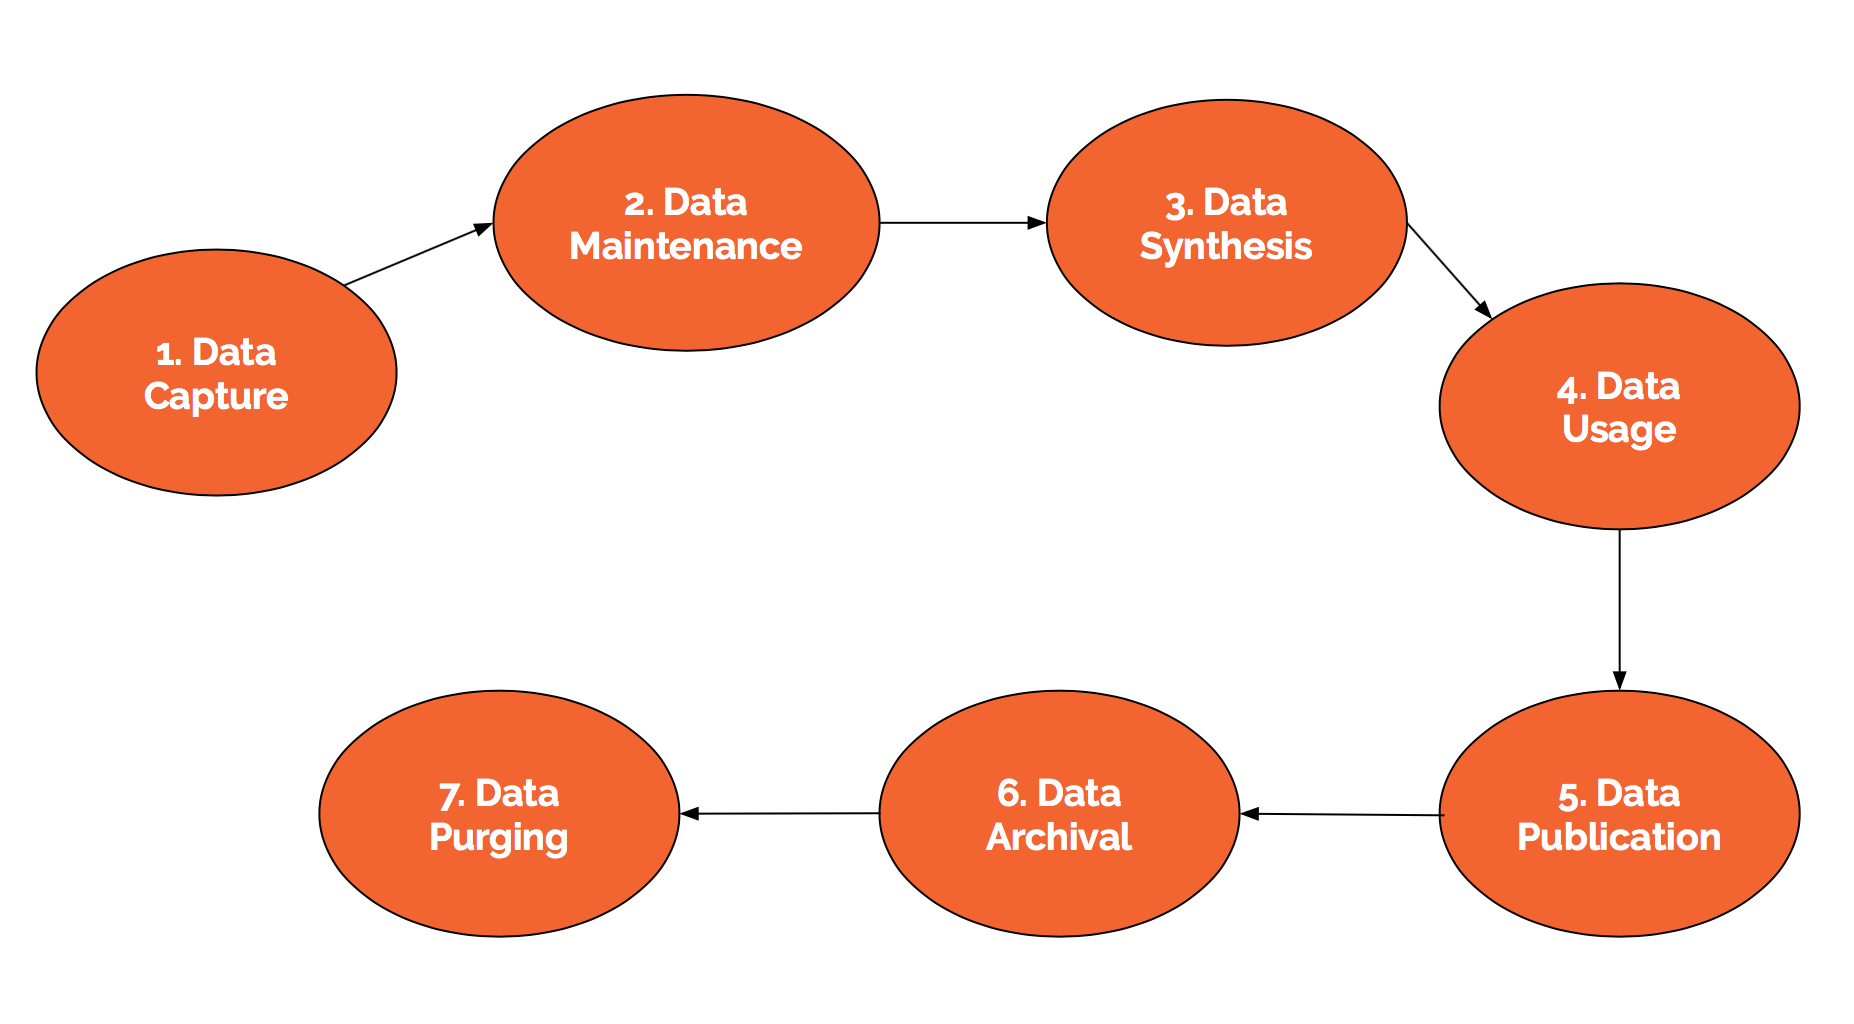
\includegraphics[height=5cm]{DataLifeCycle}
    \caption{Diagrammatic approach to the data life cycle}
    \label{fig:DataLifeCycle}
\end{figure}

The data life cycle (Figure 1 - next page) is an iterative process which describes the phases that a unit of data will pass through, from its inception to the time of destruction. Data life cycle models are important because they provide a rigid structure for considering the various operations a unit of data may undergo throughout its existence. Interestingly, it has been argued that the term "life cycle" is not actually the most appropriate term, as unlike in a regular life cycle of say, a butterfly, data will not reproduce itself to ensure continuity. There have been multiple definitions, like from Chisholm (Bloomberg) \cite{11_chisholm_2015} and from Boston University \cite{bostonDataLifeCycle}, of the data life cycle stages, with different authors having different views. This has resulted in some cases, different life cycle stages. We feel that the data life cycle proposed by Chisholm is one of the most comprehensive, hence we will use this version of the data life cycle in our paper. Refer to Figure \ref{fig:DataLifeCycle} for a diagrammatic approach to the data life cycle proposed.

\begin{enumerate}
\item \textbf{Data Capture}

This is the beginning of the data life cycle, and encapsulates the various processes involved in the creation of a unit of data. There a number of ways this happens in a system:

1. \textit{Data Acquisition}

In this method, existing data from an external system is introduced to the system under consideration. This is still considered as part of the data capture process as in the past, it didn't exist in our system; instead it only existed in an external system. This is common especially when migrating data from one system to another, or when an organization forms a joint-venture/is acquired by another.

2. \textit{Data Entry}

This method involves the manual entry of data into the system, where new data is created with the help of human operators or devices that generate data for the enterprise automatically. This is the most frequently used method in day-to-day operations.

3. \textit{Signal Reception}

In this method, the data is created by the devices as opposed to people (for example, via sensors) and have this data fed into the system for storage and processing at a later point in time. This is typically important in control systems, but with more Internet of Things devices, this form of data acquisition has become especially popular too.

\item \textbf{Data Maintenance}

This process allows for data pre-processing and involves actions like cleaning, enrichment, integration, movement, as well as things like extract-transform-load (ETL) processes. The ETL process is essentially the process where data is read, then converted from its previous form into the form it needs to be in, then written in under it'=s new format. An important idea of this phase is that no value is derived from the data itself; it is merely processed.

\item \textbf{Data Synthesis}

This stage is where semantics are extracted from the data. Deriving value from the data is extremely important, especially in big data systems due to the fact that the extremely large amounts of data allow us to identify useful and interesting patterns that may not be immediately obvious - which is something that was never possible in small data systems in the past.

It is important to note that in the data synthesis stage, inductive reasoning, as opposed to deductive, is used when deriving value from the data. For example, a case of deductive reasoning would be calculating the net sales for a business with the formula:
\[Net Sales = Gross Sales - Cost Of Manufacture \]
This particular case of deductive reasoning is trivial to solve, since as long as one knows the underlying equation, and the value of \textit{GrossSales} and \textit{CostOfManufacture}, one would be able to easily derive the \textit{NetSales} value - this is not really considered as deriving value from the data. In the case of inductive logic, modeling is needed, which takes in the large amounts of data and identifies things like patterns, which based on judgment and opinion, allows new data to be derived (for example, in the case of credit score calculations).

\item \textbf{Data Usage}

The data usage stage in the data life cycle is relatively self explanatory. In this stage, the raw, as well as the derived data is used in the operations of a particular enterprise for it to run and manage itself. However, one thing to note in particular is that in this stage, the usage of the data is contained within the enterprise itself and there is no data leakage in any form outside the bounds of the enterprise.

\item \textbf{Data Publication}

This is where the data actually leaves the owning entity and is transferred to a location external to the entity. For example, in the case of a financial institution, it may send out reports of its financial standings to its investors, or in the case of a hospital, reporting the mortality rates to a national health care database. The one thing that has to be taken into consideration is that once the data has left the owning entity, it is impossible to recall it, and a consequence is that data values cannot be amended once they have left the entity.

\item \textbf{Data Archival}

Eventually, a unit of data will reach a point where it is no longer in active use, and it is appropriate for more up-to-date information to replace it. This is especially apparent in today's data-rich environment, where in many cases, concrete data may quickly become superseded with newer values in a matter of seconds. It should be noted, though, that it is uncommon for data to be immediately deleted once it has been superseded with more up to date values. In this phase, it is typical that a unit of data is stored for a number of years but this can vary a lot depending on many other factors. One example is in the case of historical analysis, where several datasets from many different time periods need to be compared.

The data is moved over to an environment external to the active production environment in this phase. No further maintenance, usage or publication of the data takes place when the data reaches the archived environment; in the case where there is a need for any of these three actions, the data would be restored to the appropriate environment where the corresponding action takes place.

\item \textbf{Data Purging}

When a data item is no longer needed, it is considered to be useless as it has reached the end of its life, and needs to be removed. This process is known as the data purging process. This is in contrast to the process of data deletion, which is often seen as a temporary effect, however the core idea of purging is that data that is no longer needed is deleted permanently to free up some computing resources. 

\end{enumerate}

As can be observed here, the data life cycle is indeed a long process, with a number of intricacies in every step of the way; therefore, every step of the phase needs to be well-planned and well-thought-out. One of the core issues that needs to be taken into consideration is that the data life cycle handles sensitive and confidential data, hence it is critical that measures are taken at every step of the way to ensure the security of the data and the privacy of the users (or the related entities) are preserved.

%Recommendations go here
\section{5. Recommendations for preserving contextual privacy and security throughout the data life cycle}

Data handlers should be aware that there is no specific point in the data life cycle that can be attacked; instead, data is vulnerable to attacks at every step of the way. Hence, we propose a set of guidelines that should be followed every step of the way to ensure contextual privacy and security is preserved.

\begin{enumerate}
\item \textbf{Data Capture}

The data capture phase is when new data is introduced into the system. This one of the best ways we could introduce potentially malicious code or data files into the system which could affect the operations of the system. One of the most important things in this phase, regardless of the capturing method is ensuring that some form of sanitization is executed on the dataset being introduced into the system. The idea is to ensure that pure data that isn't potentially malicious is going to be introduced into the system (for example, inputting database query statements or commands in text fields, or opening executable files when data is copied over from a different system with the use of files). More specifically, there are additional measures that can be put in place for the various categories of data capture methods:


1. \textit{Data Acquisition}

When acquiring data from a different system, it is important to check the current privacy policy from the existing system; in some cases, there may be clauses in the privacy policy that disallow the transfer of the data over to a different system. For this reasoning, migration may need the explicit consent from the users/entities that have contributed their data to the old system. In the case that such clauses don't exist, it should be ensured that during the migration process, the data being copied over is encrypted in order to prevent eavesdropping parties from exploiting the raw data. It is also important to ensure that the data integrity isn't compromised in any way during transit. This can be solved by digitally signing the data prior to it being sent over, and verifying the signature on the data set on the receiving end to ensure the integrity of the data. If the signatures don't match up, then is an indication that there was some form of modification that occurred in transit. In this scenario, the data is likely untrustworthy and should be dropped on the receiving end and a request for re-transmission should be sent back to the sender system.

2. \textit{Data Entry}

In the data entry method, it is good practice to also consider the parties that are authorized to enter the data into the system. Implementing some form of an access control list would be useful in this case, where only users with the appropriate credentials would be able to access the system for data entry. From a privacy standpoint, it should be ensured that the necessary privacy notices have been presented to the entities that data was collected from, in order to ensure that the privacy of those entities aren't violated. Sanitization of input will help in this case, as it would disallow accidental entries, and ensure that there are no deliberate attempts to input invalid commands through command injections in the data fields (like SQL injections).

3. \textit{Signal Reception}

The capture of data through signal receptions also needs some additional measures to ensure that the data capture process is safeguarded, as well as the central data stores of the system. For one, the system should be designed in such a way that only approved signals are accepted, where all other unverified signals are automatically dropped. Since signals are received from devices like sensors, approved sensors (for example, only sensors of particular MAC addresses - if they are running over a network, or only sensors of certain universally unique identifiers - basically some form unique value that would describe a particular sensor) would be an accepted sensor that the system will listen to. If an unauthorized sensor attempts to connect to the system, it would automatically be dropped even if it tries to send signals to the system. Naturally, it should be ensured that only authorized users are allowed to modify the list of approved sensors.

\item \textbf{Data Maintenance}

In order to further preserve the privacy of users, as well as the security of the data stored itself, measures should be taken to ensure that the data at rest is encrypted once the necessary maintenance tasks are complete. In terms of the maintenance tasks themselves, care should be taken in order to ensure that the privacy of the users who have contributed their data to the system by removing personally identifiable information from the data being processed. This could be done as part of the extract-transform-load process, where personally identifiable information is removed from the data in the system.

In some cases, organizations still need personally identifiable information for certain tasks. For example, in a bank, they would need to still have the credit card transaction records that can be linked back to a client for billing purposes, but at the same time, they would want to use the data of all the transactions conducted by their clients to learn the most common transactions their clients conduct in order to be able to better cater their credit card offerings depending on the time of the year, for example. In a case like this, instead of deleting the personal information wouldn't make sense, nor would making a copy of all the data then deleting the personal information from one copy (space complexity would be an issue here, especially considering the extremely large amounts of data in big data systems). Instead it would be possible to have a map table that maps the unique identifier with a particular client and replacing the personal information in the transaction records with a unique identifier that doesn't reveal any information to an outside party without having access to the map table. One thing to note is that the map table has to be kept securely, so as long as only authorized personnel are allowed to access this file, and the file is kept encrypted until used, this should be adequate.
\item \textbf{Data Synthesis}

The synthesis stage is arguably the most important part of the data life cycle in a big data system, as this is where patterns are identified and actual value from the data is extracted via inductive reasoning. However, the patterns we identify or the values we derive can be very sensitive - arguably more sensitive than even the data maintenance stage. As a result of this, care has to be taken to ensure that only authorized users are allowed to have access to the data synthesis module in the system. This is not only to prevent unauthorized users from having access to the already synthesized patterns and findings, but also preventing unauthorized users from actually modifying the parameters, to use the power of the analytic modules in this stage to try and compute patterns that could affect the privacy of some users. It also prevents unauthorized users from deliberately making changes to the analytic parameters in the system that may lead to inaccurate values to be derived.

From a security standpoint, as soon as new patterns are derived, it is also necessary for them to be encrypted as well, since they likely represent much broader insights. It would be useful to pre-sign these data values created as well - so that in the case that there is a compromise of the system, and the derived values are modified, it can be tracked as the derived values would no longer tally with the signature associated with it. Sometimes, to harness more computing power, some of the analytic modules may be designed to be deployed in distributed environment. In that case, it would be necessary that a secure connection is established between two machines, and that the data is transmitted in encrypted form, and together with a signature. Again, like in the case of the data acquisition process, the signature of the data being transmitted across the systems should be verified. 

Since performance is crucial in this stage as well, one thing that could be considered is a hybrid encryption setup \cite{jbenz_hybridEnc} \cite{katz_2004} (where the expensive public key encryption is used just once to generate a symmetric key to be used later on - as this takes advantage of the less computationally expensive symmetric key encryption to encrypt the data, but allows us to still have fresh keys every time a connection is opened or after a fixed time).

\item \textbf{Data Usage}

Once new insights and patterns have been derived, they are both used in the operations of the entity. Unfortunately, this opens up a large avenue for privacy and security violations. 

Firstly, while data in this phase should still be in the entity itself (it only leaves the entity in the data publication stage), it is necessary to take precautions that prevent the data from being removed out of the entity without permission. For example, it would be possible to isolate the devices that are able to access the databases in this stage, by only giving them read access, and not allowing for external connections to these devices used to access (i.e. limiting network connections, preventing external storage devices from being connected). Once again, an access control list could be introduced to limit the users who are able to access the data stores in this stage.

Secondly, the data should be stored centrally and copies should not be stored on a local machine when the data is still in use. This may be a potential issue in some cases, as network performance between the devices used to access the data store and the data store itself can be an issue, but this can be solved with either the use of better transmission media (like fiber glass based networks, or introducing scratch disks on the local device that caches some - but not all - data and clears this cache periodically).

On the privacy front, there is also the ethical debate of whether or not it is legal to use data in the ways which organizations deem acceptable.  This is referred to as ``permitted use of data''. There may be regulatory or contractual constraints on how data may actually be used \cite{11_chisholm_2015}. In this case, it is important that the privacy policy that the user had agreed to when their data was collected in the data capture phase is referred to before the data is used in a way that may potentially compromise the contributing user's privacy. This is especially true when using raw data.

\item \textbf{Data Publication}

In the data publication stage, the main issue is the privacy of the contributing users. Hence the privacy policy that a user agreed on before data collection has to be respected. There should be additional verification that should be done, like potentially employing a multi-layer approval stage. In the case of raw data, in no way should the data be published without it being anonymized. This is something that has to be made sure especially if there was no pre-anonymization that was done in advance to the raw data. 

From a security standpoint, it is beneficial for the published data to have some form of digital signature as well, in order to ensure that if the data being published has been altered in any form after it was marked as published, it can be traced. Another enforcement would be to have some form of information rights management implemented into the files as they are being published. Information rights management (IRM), is basically like digital rights management, but for documents. It is used for managing, controlling and securing content from unwanted access, and mainly focuses on protecting sensitive data, especially data that is exchanged with parties outside an organization \cite{irm_rouse}. With IRM, it would be possible to prevent unauthorized copying or forwarding of the data being published, as well as allows us to ensure no modifications can be made to the file and only those who are permitted to access the file are the ones who are actually able to access the file - and these rules will even apply outside of the internal network of the publishing entity. This is an advantage, since if there is a need in the future to revoke access to a copy of the file, it can be done easily \cite{kohgadai_2016}.

\item \textbf{Data Archival}

As data archival can lead to data being stored for extended periods of time, with infrequent accesses, it would be reasonable to have more complex, and stronger encryption policies; processing time is no longer a priority in this stage. It is not expected that this data gets accessed very often, so the added protection by stronger encryption algorithms would be beneficial. Access to the data archives in big data systems should also be much stricter than the active environment since there is no need for many people to have access to it, compared to the active environment. Activity monitoring should be implemented as well, to track the access and operations that are conducted on the data archives by permitted users, and if possible, some form of method that alerts all system administrators when a potentially dangerous action or an attempt at an unauthorized transaction is executed by a user.

In terms of privacy, prior to archival, it is necessary to ensure the procedure is in compliance with the privacy policy. If there are provisions that disallow data to be stored on an archive drive that is potentially not within the organization in which the system resides, then this cannot be done. Also, there should be some form of tracking that is able to provide reminders when the data is approaching its expiry date or end of life date. This is to ensure that data isn't kept beyond the agreed expiry date of the data, as if there were to be a breach in the archives, not only would the system be at fault for the breach, it would also be at fault for retaining data beyond the agreed date.

\item \textbf{Data Purging}

In the data purging process, care has to be taken to ensure that purging abides by the standards set out by the relevant bodies or the data deletion policy. For example, some organizations have stipulated in their data management policy the standard of data deletion that should be used (like in the case of UC Berkeley \cite{berkeley_delete}). In the case that such policy exists, then the big data system should comply to this deletion standard. 

Assuming there is no data deletion policy currently stipulated in the organization using the big data system, then an appropriate Department of Defense Media Sanitization Guideline could be used in order to ensure secure deletion. The level of deletion that is to be used depends on the sensitivity of the data; the more sensitive the data, the more overwrites with null data should be done to purge out the data. A challenge in this phase of the data life cycle is proving that the purge has actually been done properly\cite{11_chisholm_2015}. To alleviate this, it could be possible to implement logging when the deletion takes place, so that the deletion can be tracked - one thing to note would be that the logs generated should be read only to prevent modification.

\end{enumerate}

There are some contextual privacy issues that have also arisen in recent times when the same datasets span multiple countries with differing legislation on the topic. Some authors suggest that there be a new layer in the data life cycle, called an Access Control and Accounting Infrastructure (ACAI), which is described as a trust management infrastructure \cite{demchenko2015cloud}. The motivation behind this stemmed from a primarily scientific focused infrastructure and suggests that such an infrastructure should ``protect data policy, ownership, linkage (with other datasets and newly produced scientific/research data), when providing (long term) data archiving'' \cite{demchenko2015cloud}.

%Security Violations go here

\section{6. Contextual privacy and security improvements to existing big data systems}

\subsection{Hadoop and other cluster computing frameworks}

In traditional database management systems, large datasets were becoming increasingly inconvenient to store, so new systems emerged to fulfill this requirement\cite{franklin2005databases}. Hadoop is a software framework intended for use in distributed storage and processing of large datasets\cite{white2012hadoop}. It was originally designed to unify the processing power of commodity machines with local storage to process vast amounts of data, while minimizing the costs of computing. Hadoop implements a file system called Hadoop Distributed File System (HDFS) that provides scalability and reliability of storage, by spanning large clusters of computers \cite{borthakur2008hdfs}. Three common issues are typically associated with Hadoop implementations:

1. \textit{Weak security at the core}

One drawback about many big data systems is that they were not designed with security in mind; they were largely intended to be run within trusted environments, and Hadoop is no exception. At its inception, Hadoop had not authentication for users, nor was there any concept for preservation of data privacy \cite{lublinsky2013professional}.  Although Hadoop has recently adopted best-practice security standards, its weak foundation in this area is still worrying for data managers.

2. \textit{Fragmented data}

In Hadoop, redundancy and resiliency are encouraged, which are both achieved via replication through slave nodes. Unfortunately this allows the dataset as a whole to succumb to fragmentation issues as there may be delays in the replication process. As a result, there is a lot of complexity in the system, and security issues arise due to the absence of a robust security model \cite{sharma2014securing}.

3. \textit{Distributed computing paradigm}

Since the availability of resources is necessitated by parallel processing on multiple machines of data, there simply exist more points of weakness in the entire system. Due to the eager use of data replication, the entire security of the system is reduced to the weakest node \cite{sharma2014securing}.

4. \textit{Communication between nodes}

Since Hadoop was meant to be run in a trusted environment, node to node communication does not implement any secure communication protocols, so data is transferred in the clear and thus susceptible for exploitation \cite{lakhe2014introducing}.

5. \textit{Access control in its infancy.} 

In older versions of Hadoop, for seamless integration, one of the characteristics was that all users with access to the trusted environment also had full control of the system; they could submit arbitrary code for execution. File permissions and access control lists were used in earlier distributions to mitigate this weakness, however they were relatively weak, as the access control mechanism was easily evaded; users could impersonate any other, and exploit privileged actions.

In addition, users of the system had the same level of access across clusters, and any user could access and modify any dataset, which obviously yielded opportunities for data misappropriation. Luckily as Hadoop grew in popularity, security professional began to express concerns about the insider threats looming over the entire system and implemented a robust authentication system called Kerberos \cite{o2010integrating}. However, since Kerberos only provides authentication services, it is not a solution for data at rest.

\subsection{Security issues in MongoDB and various NoSQL databases}

MongoDB is a popular document-oriented example of a NoSQL database that has seen much popularity in recent times. It offers a ton of advantages over traditional relational database systems, including consistency and partition tolerance. It stores data as documents (usually in JSON format) and models data in a hierarchical manner \cite{banker2011mongodb}, which is more intuitive for modern programming practices like object-oriented programming. It provides very high availability and scalability by using sharding and replication \cite{membrey2011definitive}. Sharding is a method for distributing data across across machines, while replication refers to copying data across machines to increase redundancy and data availability. Some existing MongoDB security issues include:

1. \textit{Data at rest is unencrypted by default} 

The most glaring issue with MongoDB is that its data storage system is completely unencrypted by default \cite{okman2011security}. Like Hadoop, MongoDB, and many NoSQL databases were designed to be run within a trusted environment. In the case of unencrypted data, this means that malicious parties that have physical or virtual access to the file system can extract information as they please. Unfortunately, MongoDB is largely reliant on the client code for encryption of any sensitive information before it saves to the database. Some mitigation techniques for this scheme include implementing proper file system permissions and file system level encryption \cite{okman2011security}.

2. \textit{Susceptibility to injection attacks}

Similar to relational databases that support query languages, MongoDB is also susceptible to injection attacks, albeit of a different kind \cite{sullivan2011server}. MongoDB is highly reliant on JavaScript as its scripting language. The commands available to developers are implemented as JavaScript programs, and by default, server-side execution is enabled, leaving the system susceptible to injection attacks. All injection attacks are caused by poor means of sanitization, thus a good recommendation is to implement well-tested third party libraries for new development, which greatly reduces the risk of introducing security bugs \cite{ron2016analysis}.

\section{7. Existing solutions}

There have been many suggestions by the big data community relevant to the goals of this paper. Some existing solutions that preserve privacy on big data systems include:

1. \textbf{Privacy-preserving, attribute-based, fine-grained access control \cite{nabeel2013privacy}.}

One way of protecting confidentiality of data is by using encryption. However, this alone may not be sufficient to protect users' privacy, as data handlers often need to enforce things such as identity attributes like user roles, and preferences. These systems are known as attribute-based systems, where fine-grained access control is a requirement, and based on policies specified using identity attributes. The gist of this idea is that the system can process data relative to sensitive information without actually knowing the semantics of the data itself, thereby preserving the confidentiality of certain details.

Nabeel et. al provide a context-based publish subscribe model for distributed communication commonly found in big data systems \cite{nabeel2013privacy}. Their architectural pattern is an improvement on the existing publish-subscribe systems, because it performs an evaluation of blinded subscriptions against blinded notifications without decryption. They do note that there is a hit to routing efficiency.

2. \textbf{Policy languages.}

There has been a lot of work in extending rudimentary access control systems, providing responses beyond a simple ``yes/no'' \cite{hull2004enabling}; these are known as policy languages, and they provide more expressive power than traditional mechanisms. Some authors believe that policy languages such as XACML represent good solutions for fine granular access control \cite{demchenko2013big}. XACML is a standard for fine-grained access control and authorization systems. It defines a policy language for access control, accompanied by an architecture and a processing model that follows the rules defined in the policies. XACML is based on that principle that authorization features should be based not only on the request context attributes like subjects/users, but also on the structured data content. A promising direction is a design that applies attribute based access control mechanism with policies that incorporate data granularity. These policies may contain complex logical expression based on the attributes. Unfortunately, for larger and more complex datasets, XACML may not be a great solution, as there is some overhead of the format, which may be problematic for the volume and velocity of big data systems.

3. \textbf{Access control in NoSQL databases.}

The recently popular NoSQL implementations such as Cassandra, MongoDB, and Accumulo provide varying levels of security and access control \cite{demchenko2013big}. Unfortunately, most implementations have coarse-grained authorization features. Out of the three, however, Accumulo provides the most support, however it is still at its early development stage, and has poor support for distributed and multi-domain environments \cite{demchenko2013big}.

4. \textbf{Open source middleware systems.} 

Middleware is any software that sits between the machine's operating system and its applications, while providing services to the latter. Some existing initiatives such as the European Union's platform, FI-WARE, address privacy in big data systems with optional authorization and authentication mechanisms that include a policy language to define the attributes and credentials required to access resources \cite{skarmeta2013internet}. They also include a data handling policy language and it is typical that it defines how data attributes and credentials are handled, and to whom they are passed on, which is crucial for contextual privacy. In addition, they provide the means to release and verify the given attributes and credentials.

5. \textbf{Encryption for data at rest.}

The aforementioned mechanisms are sufficient to ensure no violations of sensitive information occur at several stages of the life cycle, such as the data access, transfer and processing stages \cite{demchenko2013big}. However, the issues with regular access control systems remain: the setup is that a trusted server mediates the access control. Unfortunately if this trusted server is compromised, then the confidentiality of the data will be as well. These techniques ensure that in the worst-case scenario where a server is compromised, the data itself is ensured to preserve integrity. These schemes are great for data at rest, and is especially relevant to many use cases in big data, especially healthcare or distributed sensor networks. A potential solution to this is to use encryption enhanced access control policies that provide an extra layer on top of traditional access control schemes, i.e. attributes based encryption. These extra features ensure that data decryption only occurs for the targeted subject or attribute owner, which is a sufficient condition for contextual policy protection \cite{goyal2006attribute}.

6. \textbf{Data anonymization.}

There are some suggestions from the community that data anonymization is a potential solution for protecting contextual privacy \cite{cormode2009anonymized}. The idea is that in the worst-case, if context violations were to occur, the damage would be minimized since the data is obfuscated. Some researchers believe that this path is futile, such as Montjoye et al\cite{de2013unique}. In their experiments, a mobility dataset of 1.5 million users was collected over a 15 month period and even after obfuscating personal information such as phone numbers, unique IDs, and names, they still managed to identify a person with 95\% accuracy using spatial-temporal data points. In another scenario, chunks of the Netflix challenge dataset were re-identified using an external data source (the IMDB database) \cite{narayanan2008robust}.

\section{8. Conclusion}

With the emergence of the big data paradigm, context can be exploited in a myriad of novel ways as the relevant datasets transition between states. Security and privacy in such systems are more important than ever, and as such this paper surveyed the key challenges and recommendations in big data systems against the data life cycle model. Although many existing implementations were built on shaky foundations of security and privacy, they have since seen rapid and tremendous improvements in this regard. We explored some successfully adopted solutions, such as access control systems, middleware, and policy languages that are sufficient for preserving the confidentiality of a unit of data in the myriad of states it transitions through. The adoption of these new security and privacy techniques in real world implementations is comforting, however should be approached with caution as they are still in their infancy.

Upon surveying the state of solutions relevant to this paper's goal, our suggestion to the community is that the best defense against data misappropriation is awareness. For privacy in modern big data systems, due diligence about the semantics of the data is key, as well as robust access control systems, which becomes more important as the number of users in the system increases. When it comes to security, the support is mostly there. For systems where it ceases to exist, there is no doubt they will reach that state eventually, as vendors have been very proactive in this area recently. Unfortunately, the default state of many implementations is not geared towards contextual security, thus our recommendation to readers is to be cognizant of the many configurations available for the employed technologies, and to stay informed about the inherent weaknesses in these systems.

%
{\footnotesize \bibliographystyle{IEEEtranS}
\bibliography{reference}}

 \end{document}